\chapter{Spanning Tree Construction}

\begin{definizione}[Spanning Tree]
    Un albero ricoprente (Spanning Tree) di un grafo $G = (V, E)$ è un sottografo connesso e aciclico di $G$ tale che $T = (V, E')$ dove $E' \subseteq E$ . In altre parole è un albero che include tutti i nodi di $V$.
\end{definizione}

\begin{definizione}[SPT Construction Distributed Problem]
    In un sistema distribuito, il problema di costruire un albero ricoprente (Spanning Tree) del grafo $G = (V, E)$ significa portare il sistema da uno stato iniziale, in cui ogni nodo è consapevole solo di se stesso e dei suoi vicini, a uno stato finale in cui tutti i nodi sono organizzati in una struttura ad albero che copre tutti i nodi del grafo. In altre parole,
    \begin{description}
        \item[Configurazione Iniziale:] Ciascun nodo $x \in \mathcal{E} = V$ mantiene una struttura dati $\texttt{tree\_neigh(x)} = \emptyset$. La possiamo immaginare come un vettore binario, dove ogni posizione rappresenta un nodo vicino ad $x$, e il valore 1 indica che l'arco tra $x$ e quel nodo è parte dell'albero, mentre 0 indica che non lo è.
        \item[Configurazione Finale:] $\forall x \in \mathcal{E} = V$, 
        \[
            \texttt{tree\_neigh(x)} = \{\text{archi che appartengono allo ST}\},
        \]
        e l'unione di tutti questi insiemi per  forma un albero ricoprente del grafo $G$. 
    \end{description}
\end{definizione}

Il problema è formalizzato dalla triplia $P = \langle P_{init}, P_{final}, R \rangle$, dove:
\begin{description}
    \item[$P_{init}$] = $\forall x \in V$, 
    \begin{align*}
        &\texttt{tree\_neigh(x)} = \emptyset \\
        &\exists! s \in V,\ state(s) = \texttt{initiator} \\
        &\forall x \in V \setminus \{s\},\ state(x) = \texttt{idle}
    \end{align*}
    \item[$P_{final}$] = $\forall x \in V$, 
    \begin{align*}
        &\texttt{tree\_neigh(x)} = \{y \in N(x): (x, y) \in E'\} \\
        &\bigcup_{x \in V} \texttt{tree\_neigh(x)} = T(V, E') \text{ albero ricoprente del grafo } G \\
        &\forall x \in V,\ state(x) = \texttt{done}
    \end{align*}
    \item[$R$] = $\{\texttt{TR, BL, CN, UI}\}$
\end{description}

Quindi, a differenza di un algorimo centrallizzato (Kruskal, Prim), la conoscenza dello ST è distribuita tra i nodi, e ogni nodo deve collaborare con i suoi vicini per costruire l'albero ricoprente. Non esiste quindi una visiione globale dell'albero, ma ogni nodo deve basarsi solo sulle informazioni locali e sui messaggi ricevuti dai suoi vicini per decidere se includere o meno un arco nel suo insieme $\texttt{tree\_neigh(x)}$.

\section{Single Source SHOUT Protocol}

L'idea dell'algoritmo è quella di chiedere ai nodi vicini se sono interessati a far parte dello ST, e se sì, includere l'arco che li collega al nodo che ha fatto la richiesta. In questo modo, partendo da un nodo iniziale (initiator), si costruisce gradualmente lo ST coinvolgendo i nodi vicini.

Definiamo $\Sigma = \{\texttt{initiator}, \texttt{idle}, \texttt{active}, \texttt{done}\}$ dove $S_{init} = \{\texttt{initiator}, \texttt{idle}\}$ l'insieme dei stati iniziali e $S_{final} = \{\texttt{done}\}$ l'insieme dei stati finali.

\begin{itemize}
    \item Inizialmente, tutti i nodi tranne l'iniziatore $s$ sono in stato \texttt{idle}, e $s$ è in stato \texttt{initiator}. Spontaneamnete, $s$ si sveglia e invia i messaggi di domanda (\texttt{Q}) a tutti i suoi vicini, proponendo loro di essere connessi a lui nello ST (cioè essere suoi figli).
    \item Quando un nodo $x$ nello stato \texttt{idle} riceve un messaggio \texttt{Q}, questo si attiva, sceglie come padre il \textbf{primo} nodo da cui ha ricevuto il messaggio e invia a tale nodo il messaggio \texttt{YES}.
    \item Successivamente, $y$ invia a tutti i suoi vicini, tranne il padre, un messaggio \texttt{Q} per chiedere se vogliono essere suoi figli. Se un nodo $z$ nello stato \texttt{active} riceve un messaggio \texttt{Q} da $y$, risponde con un messaggio \texttt{NO} perché ha già scelto un padre e non può accettare più di uno. Se invece $z$ è nello stato \texttt{idle}, risponde con un messaggio \texttt{YES} e si attiva, scegliendo $y$ come padre.
    \item Ogni nodo conta il numero di risposte ricevute da suoi vicini. Quando un nodo $x$ ha ricevuto risposte da tutti i suoi vicini, passa allo stato \texttt{done} e non fa più nulla.
\end{itemize}

Per un nodo $x$, i vicini che rispondono con \texttt{YES} saranno inclusi nel suo insieme \\ $\texttt{tree\_neigh(x)}$ includendo anche il vicino che ha fatto la richiesta.

Possimo quindi considerare il protocollo SHOUT come un broadcast con reply.

\begin{algorithm}[H]
\caption{Algoritmo di SHOUT}
    \begin{algorithmic}
    \If{state(x) = \texttt{initiator}} spontaneously
        \State root $\gets$ true
        \State \texttt{tree\_neigh(x)} $\gets \emptyset$
        \State state(x) $\gets$ \texttt{active}
        \State counter $\gets 0$
        \ForAll{$v \in N(x)$}
            \State send(\texttt{Q}, $v$)
        \EndFor
    \EndIf
    \State
    \If{state(x) = \texttt{idle}}
        \State $\texttt{Q} \gets$ receive()
        \State \texttt{tree\_neigh(x)} $\gets \{ \texttt{sender} \}$
        \State root $\gets$ false
        \State counter $\gets 1$
        \State send(\texttt{YES}, \texttt{sender})
        \If {counter $= |N(x)|$}
            \State state(x) $\gets$ \texttt{done}
        \Else        
            \ForAll{$v \in N(x) \setminus \{\texttt{sender}\}$}
                \State send($\texttt{Q}$, $v$)
            \EndFor
            \State state(x) $\gets$ \texttt{active}
        \EndIf
    \EndIf
    \State
    \If{state(x) = \texttt{active}}
        \State $\texttt{reply} \gets$ receive()
        \If {reply = \texttt{YES}}
            \State \texttt{tree\_neigh(x)} $\gets$ \texttt{tree\_neigh(x)} $\cup$ \{\texttt{sender}\}
            \State counter $\gets$ counter + 1
            \If {counter $= |N(x)|$}
                \State state(x) $\gets$ \texttt{done}
            \EndIf
        \EndIf
        \State
        \If {reply = \texttt{NO}}
            \State counter $\gets$ counter + 1
            \If {counter $= |N(x)|$}
                \State state(x) $\gets$ \texttt{done}
            \EndIf
        \EndIf
        \State
        \If {reply = \texttt{Q}}
            \State send(\texttt{NO}, \texttt{sender})
        \EndIf
    \EndIf
    \end{algorithmic}
\end{algorithm}

\begin{figure}[ht!]
    \centering
    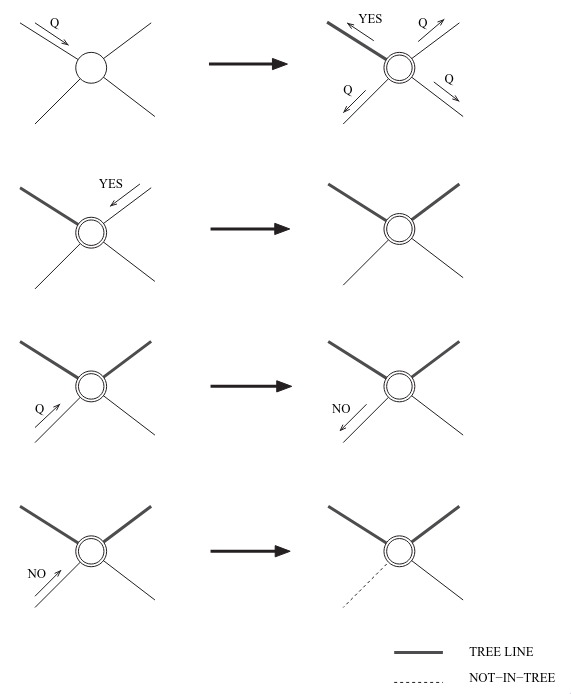
\includegraphics[width=0.5\linewidth]{images/shout.png}
    \caption{Insieme di regole del protocollo SHOUT.}
    \label{fig:shout}
\end{figure}

\subsection{Terminazione}
Il protocollo SHOUT è molto simile al protocollo di broadcast con l'aggiunta dei messaggi di reply \texttt{YES} e \texttt{NO}. Poiche siamo sotto le assunzioni \texttt{TR} e \texttt{CN}, allora ogni nodo $x \neq s$ riceverà entro un tempo finito un messaggio \texttt{Q} da un vicino, e quindi si attiverà impostando il contatore a 1 (per la correttezza del protocollo di broadcast). Per ogni richiesta ricevuta, i nodi risponderanno con un messaggio \texttt{YES} o \texttt{NO}, di conseguenza, ogni nodo riceverà (per la \texttt{TR} e per la costruzione del protocollo, ogni nodo risponderà a tutte le richieste) un numero finito di risposte ($|N(x)|$), e quindi, entro un tempo finito, ogni nodo raggiungerà lo stato \texttt{done}, terminando localmente la popria esecuzione.

\subsection{Correttezza}

Per dimostrare la correttezza del protocollo SHOUT, dobbiamo mostrare che alla fine dell'esecuzione, l'insieme di archi scelti da tutti i nodi forma un albero ricoprente del grafo $G$.

\begin{lemma}[Coerenza]\label{lemma:coerenza}
    Siano $x$ e $y$ due nodi vicini in $G$. Se $x$ ha come vicino $y$ in ST, cioè $y \in \texttt{tree\_neigh(x)}$, allora $x$ è vicino di $y$ in ST, cioè $x \in \texttt{tree\_neigh(y)}$. Quindi 
    \[
        \forall x, y \in V,\ y \in \texttt{tree\_neigh(x)} \iff x \in \texttt{tree\_neigh(y)}.
    \]
    \begin{proof}
        Supponiamo che $y \in \texttt{tree\_neigh(x)}$. Allora $y$ ha risposto con un messaggio \texttt{YES} alla richiesta di $x$, e quindi $y$ ha scelto $x$ come padre. Ma se $y$ ha riposto con \texttt{YES} a $x$, allora $y$ era nello stato \texttt{idle} quando ha ricevuto la richiesta da $x$ e per definizione del protocollo $y$ inserisce $x$ nel suo insieme $\texttt{tree\_neigh(y)}$. Quindi $x \in \texttt{tree\_neigh(y)}$. La dimostrazione dell'implicazione inversa è simile, con $x$ e $y$ scambiati.
    \end{proof} 
\end{lemma}

\begin{lemma}[Connettività/Spanning]\label{lemma:spanning}
    Il sottografo $T = (V, E')$ definito da 
    \[
        E' = \bigcup_{x \in V} \texttt{tree\_neigh(x)}
    \]
    è connesso e include tutti i nodi di $V$. In altre parole, il sottografo indotto dagli archi su cui è viaggiato il messaggio \texttt{YES} è connesso e include tutti i nodi di $V$ (è ricoprente e connesso).
    \begin{proof}
        Vogliamo dimostrare che per ogni nodo $x \in V \setminus \{s\}$, se $x$ ha risposto \texttt{YES} ad un nodo $y$, allora $x \in \texttt{tree\_neigh(y)}$, dove quest'ultimo è connesso alla sorgente $s$ tramite una sequenza di archi sui quali sono passati i messaggi \texttt{YES}, e tale sequenza formerà un cammino da $s \to x$.
        
        Sia $x$ un nodo qualsiasi in $V \setminus \{s\}$. Se $x$ ha risposto \texttt{YES} ad un nodo $y$, allora $x \in \texttt{tree\_neigh(y)}$, e dato che $y$ deve aver inviato una proposto al nodo $x$, allora $y$ si trova in \texttt{active} alla ricezione della risposta \texttt{YES} da $x$. Ma $y$ invia una proposta al nodo $x$ solo se:
        \begin{itemize}
            \item $y$ è la sorgente $s$, e quindi è connesso a se stesso, oppure
            \item $y$ ha ricevuto una proposta da un nodo $z$ e ha risposto \texttt{YES} a $z$, e quindi $y$ è connesso a $z$ tramite un arco su cui è passato un messaggio \texttt{YES}, quindi 
            \[
            z \in \texttt{tree\_neigh(y)} \text{ e } y \in \texttt{tree\_neigh(z)} \qquad \autoref{lemma:coerenza}
            \]
            Iterando questo processo fino alla sorgente $s$, si ottiene un cammino che collega $s$ a $x$ tramite archi su cui sono passati messaggi \texttt{YES}, e quindi $x$ è connesso a $s$.
        \end{itemize}
    \end{proof}
\end{lemma}

\begin{lemma}[Aciclicità]\label{lemma:acyclicity}
    Il sottografo $T = (V, E')$ definito da 
    \[
        E' = \bigcup_{x \in V} \texttt{tree\_neigh(x)} \text{ è aciclico}.
    \]
    \begin{proof}
        Supponiamo per assurdo che $T$ contenga un ciclo. Allora esiste una sequenza di nodi $v_1, v_2, \ldots, v_k$ con $k \geq 3$ tale che $(v_i, v_{i+1}) \in E'$ (ossia $v_i$ è padre di $v_{i+1}$) per ogni $i = 1, 2, \ldots, k-1$ e $(v_k, v_1) \in E'$. 

        Poichè ogni nodo, eccetto la sorgente invia \textbf{un solo} messaggio \texttt{YES}, allora il ciclo $v_1, v_2, \ldots, v_k$ non contiene la sorgente $s$. Per il \autoref{lemma:spanning}, deve esistere un cammino da $s$ a qualsiasi nodo, inclusi quelli de ciclo. Ma poiché deve esistere un cammino da $s$ a $v_i$, allora esiste un cammino da $s$ a $v_i$ che passa attraverso il ciclo, il che implica che esiste un cammino da $s$ a $v_i$ che contiene un ciclo. Questo è una contraddizione, poiché un cammino non può contenere un ciclo. Quindi, il sottografo $T$ deve essere aciclico.
    \end{proof}
\end{lemma}

\begin{teorema}
    Il protocollo SHOUT costruisce un albero ricoprente del grafo $G$.
    \begin{proof}
        Dal \autoref{lemma:spanning} sappiamo che il sottografo $T$ è connesso e include tutti i nodi di $V$, e dal \autoref{lemma:acyclicity} sappiamo che $T$ è aciclico. Quindi, combinando questi due risultati, possiamo concludere che $T$ è un albero ricoprente del grafo $G$.
    \end{proof}
\end{teorema}

\subsection{Message Complexity}

Come menzionato sopra, il protocollo \texttt{SHOUT = Flood + Reply}. Quindi la complessità in termini di messaggi consiste nell'esecuzione di \texttt{Flood(Q)} più le risposte \texttt{YES} o \texttt{NO} per ogni richiesta ricevuta. In altre parole,
\[
    M[\texttt{SHOUT}] = M[\texttt{Flood(Q)} + \texttt{Reply}] = 2M[\texttt{Flood(Q)}] = O(4|E|) = O(|E|).
\]
Più precisamente, i messaggi inviati dal protocollo possono essere divisi in due categorie: \texttt{Q} e \texttt{Reply} = \{ \texttt{YES}, \texttt{NO} \}. Di conseguenza, abbiamo le seguenti casistiche:
\begin{itemize}
    \item Per ogni arco $(x, y) \in ST$ costruito dal protocollo passano due messaggi: un messaggio \texttt{Q} inviato da $x$ a $y$ e un messaggio \texttt{YES} inviato da $y$ a $x$. Il numero di archi sono $|E'| = |V| - 1$, quindi il numero di messaggi in questa categoria è $2(|V| - 1) = 2(n - 1)$.
    \begin{center}
        \begin{tikzpicture}[
            node distance=3cm, 
            every node/.style={circle, draw, minimum size=0.6cm, thick},
            arrow style/.style={-{Stealth[scale=1.2]}, thick}
        ]

        \node (A) {};
        \node (B) [right of=A] {};

        \draw[thick] (A) -- (B);

        \draw[arrow style] (A) to [bend left=45] node[draw=none, above, text=red] {Q} (B);

        \draw[arrow style] (B) to [bend left=45] node[draw=none, below, text=red] {YES} (A);
        \end{tikzpicture}
    \end{center}
    \item Per ogni arco $(x, y) \in E \setminus ST$ passano quattro messaggi: due messaggi \texttt{Q} in entrambe le direzioni, seguiti da due messaggi \texttt{NO} in entrambe le direzioni. Il numero di archi in questa categoria è $|E| - |E'| = |E| - (|V| - 1)$, quindi il numero di messaggi in questa categoria è $4(|E| - (|V| - 1)) = 4(m - n + 1)$.
    \begin{center}
        \begin{tikzpicture}[
            node distance=3cm, 
            every node/.style={circle, draw, minimum size=0.6cm, thick},
            arrow style/.style={-{Stealth[scale=1.2]}, thick}
        ]

        \node (A) {};
        \node (B) [right of=A] {};
        \node (C) [right of=B] {};
        \node (D) [right of=C] {};

        \draw[thick] (A) -- (B);
        \draw[thick] (C) -- (D);

        \draw[arrow style] (A) to [bend left=45] node[draw=none, above, text=red] {Q} (B);
        \draw[arrow style] (B) to [bend left=45] node[draw=none, below, text=red] {Q} (A);
        \draw[arrow style] (C) to [bend left=45] node[draw=none, above, text=red] {NO} (D);
        \draw[arrow style] (D) to [bend left=45] node[draw=none, below, text=red] {NO} (C);
        \end{tikzpicture}
    \end{center}
\end{itemize}

\textbf{Osservazione.} Su ogni arco $(x, y)$ non potranno mai passare le coppie di messaggi (\texttt{NO}, \texttt{YES}) e (\texttt{YES}, \texttt{YES}).

\begin{description}
    \item [(\texttt{NO}, \texttt{YES})] Non può accadere in quanto il nodo sinitro per rispondere a \texttt{NO} deve prima aver ricevuto una richiesta dal nodo destro, ma per inviare una richiesta, il nodo destro deve avere già un padre, dunque non può rispondere con \texttt{YES} a nessuna richiesta.
    \item [(\texttt{YES}, \texttt{YES})] Non può accadere in quanto due nodi per inviarsi reciprocamente un messaggio \texttt{YES} devono essersi entrambi inviati reciprocamente un messaggio \texttt{Q}, ma ciò implica che hanno già un padre, e quindi hanno già risposto con un messaggio \texttt{YES} a un altro nodo.
\end{description}

\begin{center}
        \begin{tikzpicture}[
            node distance=3cm, 
            every node/.style={circle, draw, minimum size=0.6cm, thick},
            arrow style/.style={-{Stealth[scale=1.2]}, thick}
        ]

        \node (A) {};
        \node (B) [right of=A] {};
        \node (C) [right of=B] {};
        \node (D) [right of=C] {};

        \draw[thick] (A) -- (B);
        \draw[thick] (C) -- (D);

        \draw[arrow style] (A) to [bend left=45] node[draw=none, above, text=red] {NO} (B);
        \draw[arrow style] (B) to [bend left=45] node[draw=none, below, text=red] {YES} (A);
        \draw[arrow style] (C) to [bend left=45] node[draw=none, above, text=red] {YES} (D);
        \draw[arrow style] (D) to [bend left=45] node[draw=none, below, text=red] {YES} (C);
        \end{tikzpicture}
    \end{center}

Quindi, il numero totale di messaggi è:
\[\]
\[
    M[\texttt{SHOUT}] = 2(n - 1) + 4(m - n + 1) = 4m - 2n + 2 = O(|E|).
\]

\newpage
\section{Single Source SHOUT+ Protocol}

Si osserva che nel protocollo SHOUT, i messaggi di risposta \texttt{NO} non sono necessari per far sapere al nodo che ha inviato la richiesta quando entrare nello stato \texttt{done}. Infatti, se un nodo $y$ invia \texttt{NO} ad $x$, allora $y$ ha inviato un messaggio \texttt{Q} ad $x$ prima dell'invio di \texttt{NO}, in quanto $y$ per inviare \texttt{NO} deve trovarsi nello stato \texttt{active}, e per trovarsi nello stato \texttt{active}, il nodo $y$ deve avere già scelto un nodo come padre e aver mandato il messaggio \texttt{Q} a tutti i suoi vicini. Dunque il nodo $x$ può interpretare il messaggio \texttt{Q} inviato da $y$ come un messaggio \texttt{NO}, e quindi non è necessario inviare un messaggio \texttt{NO} esplicito. 

In questa maniera, la message complexity del protocollo SHOUT si riduce a 
\[
    M[\texttt{SHOUT+}] = 2(n - 1) + 2(m - n + 1) = 2m = O(|E|).
\]

Riguardo la terminazione locale del protocollo, ogni nodo sa che il suo compito è terminato nel momento in cui passa nello stato \texttt{done}. Sarebbe interessante sapere se un nodo è in grado di capire quanto il processo termina globalmente, cioè quando tutti i nodi sono nello stato \texttt{done}. Certamente, se la sorgente è $s$ è in grado di sapere quanto lo spanning tree è completato, allora potrebbe mandare una notifica in broadcast a tutti i nodi e avvertirli della terminazione globale. Il problema è che ogni nodo ha solamente una \textbf{visione locale} della rete in cui si trova, perciò a meno che non ci sia un nodo che riesca ad osservare lo stato della rete dall'alto non è possibile sapere solo col protocollo \texttt{SHOUT/SHOUT+} quando il processo è terminato globalmente.

\textbf{Osservazione.} Osserviamo che anche nel caso della costruzione dello spanning tree, il lower bound $\Omega(m)$ è rispettato, in quanto per costruire lo spanning tree è necessario che ogni nodo riceva almeno un messaggio da ogni vicino, e quindi è necessario che ogni arco venga attraversato da almeno un messaggio.

\textbf{Osservazione.} Si può osservare che lo spanning tree costruito dal protocollo \texttt{SHOUT/SHOUT+} dipende fortemente dalla singola esecuzione e non dal protocollo, in quanto i ritardi di trasmissione variano ogni volta. Ciò implica che maneggiando adeguatamente i ritardi di trasmissione potrebbe accadere che $diam(ST) >> diam(G)$.

\begin{teorema}
    L'esecuzione di ogni protocollo di \texttt{Broadcast} costuisce uno spanning tree \textbf{entrante} (ogni nodo possiede solamente informazioni su chi è il nodo padre, generando un albero orientato verso la radice) del grafo $G$.
    \begin{proof}
        Diamo un'idea della dimostrazione. Definiamo
        \[
        father(x) = \text{ il nodo dal quale } x \text{ ha ricevuto per primo il messaggio } m
        \]
        Allora, se consideriamo l'ordinamente \textit{parziale} $father(x) > x$ otteniamo uno spanning tree entrante, con radice $s$.
    \end{proof}
\end{teorema}

\begin{algorithm}[H]
\caption{Algoritmo di SHOUT}
    \begin{algorithmic}
    \If{state(x) = \texttt{initiator}} spontaneously
        \State root $\gets$ true
        \State \texttt{tree\_neigh(x)} $\gets \emptyset$
        \State state(x) $\gets$ \texttt{active}
        \State counter $\gets 0$
        \ForAll{$v \in N(x)$}
            \State send(\texttt{Q}, $v$)
        \EndFor
    \EndIf
    \State
    \If{state(x) = \texttt{idle}}
        \State $\texttt{Q} \gets$ receive()
        \State \texttt{tree\_neigh(x)} $\gets \{ \texttt{sender} \}$
        \State root $\gets$ false
        \State counter $\gets 1$
        \State send(\texttt{YES}, \texttt{sender})
        \If {counter $= |N(x)|$}
            \State state(x) $\gets$ \texttt{done}
        \Else        
            \ForAll{$v \in N(x) \setminus \{\texttt{sender}\}$}
                \State send($\texttt{Q}$, $v$)
            \EndFor
            \State state(x) $\gets$ \texttt{active}
        \EndIf
    \EndIf
    \State
    \If{state(x) = \texttt{active}}
        \State $\texttt{reply} \gets$ receive()
        \If {reply = \texttt{YES}}
            \State \texttt{tree\_neigh(x)} $\gets$ \texttt{tree\_neigh(x)} $\cup$ \{\texttt{sender}\}
            \State counter $\gets$ counter + 1
            \If {counter $= |N(x)|$}
                \State state(x) $\gets$ \texttt{done}
            \EndIf
        \EndIf
        \State
        \If {reply = \texttt{Q}}
            \State counter $\gets$ counter + 1
            \If {counter $= |N(x)|$}
                \State state(x) $\gets$ \texttt{done}
            \EndIf
        \EndIf
    \EndIf
    \end{algorithmic}
\end{algorithm}

\newpage

\section{Multiple Sources Spanning Tree Construction}

Supponiamo ora di avere più nodi \texttt{initiator}, ossia che 
\[
    \exists I \subseteq V,\ |I| > 1 \text{ e } \forall s \in I,\ state(s) = \texttt{initiator}.
\]
In questo scenario, l'insieme delle restrizioni diventa $R = \{\texttt{TR, BL, CN}\}$

\begin{teorema}\label{th:MultipleSourcesST}
    Sotto le assunzioni $R = \{\texttt{TR, BL, CN}\}$, il problema della costruzione di spanning tree con multipli \texttt{initiator} non è deterministicamente risolvibile.
    \begin{proof}
    Consideriamo una clique di 3 nodi $x, y, z$, tutti e tre \texttt{initiator}. Consideriamo il caso sincrono in cui tutti si attivano e iniziano il protocollo al tempo $t_0$.

    \begin{center}
        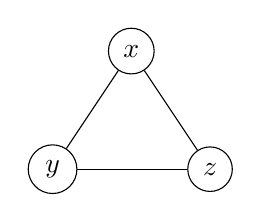
\begin{tikzpicture}
            \node[circle, draw] (x) at (1, 1.5) {$x$};
            \node[circle, draw] (y) at (0, 0) {$y$};
            \node[circle, draw] (z) at (2, 0) {$z$};
            \draw (x) -- (y);
            \draw (y) -- (z);
            \draw (z) -- (x);
        \end{tikzpicture}
    \end{center}
    Sappiamo che se prendiamo dei nodi aventi lo stesso stato interno $\sigma(v, t)$, allora essi da quel momento in poi si comporteranno allo stesso modo, dato che nessuno è in grado di distinguire una loro \textit{identità} all'interno della rete. In questo caso, al tempo $t_0$, abbiamo che $\sigma(x, t_0) = \sigma(y, t_0) = \sigma(z, t_0) = \texttt{initiator}$, e quindi $x, y, z$ si comporteranno allo stesso modo. Quindi ciascun nodo invierà un messaggio \texttt{Q} ed entrerà nello stato \texttt{active}. Quando  riceveranno un messaggio \texttt{Q} da ciascuno dei loro vicini, risponderanno con un messaggio \texttt{NO} a ciascuno dei loro vicini, e quindi entreranno nello stato \texttt{done}. Quindi, alla fine dell'esecuzione, avremo che 
    \[
        \texttt{tree\_neigh(x)} = \texttt{tree\_neigh(y)} = \texttt{tree\_neigh(z)} = \emptyset,
    \]
    e quindi non è stato costruito alcun albero ricoprente del grafo $G$.
    \end{proof}
\end{teorema}

Per risolvere questo problema è necessario risolvere un'altro problema: il problema della \textbf{leader election}. Eletto un leader tra tutti i nodi \texttt{initiator}, esso potrà eseguire uno dei protocolli di costruzione di spanning tree a singola sorgente già noti.

Vedremo in futuro che il problema della leader election può essere risolto in maniera deterministica solamente se i nodi sono univocamente identificati in maniera globale